\begin{center}
    \begin{figure}[H]
        \centering

        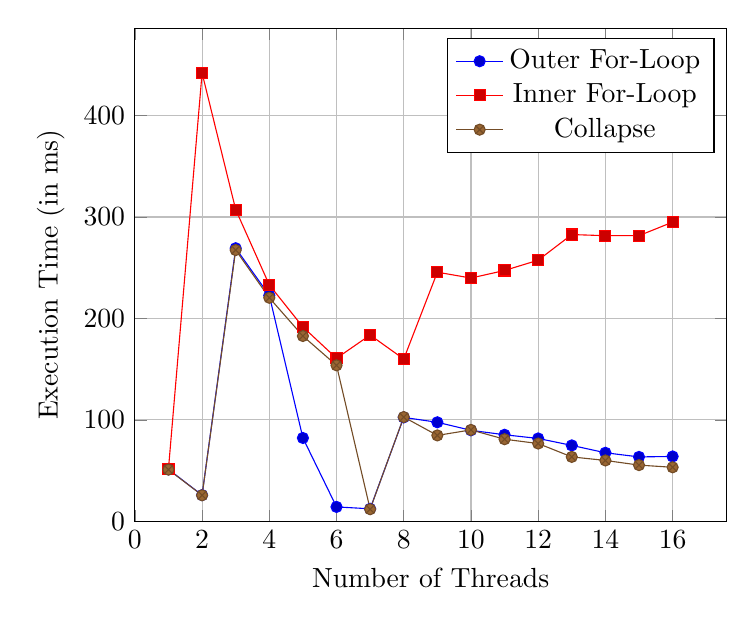
\begin{tikzpicture}
            \begin{axis}[
                title={},
                width=0.75\textwidth,
                xlabel={Number of Threads},
                ylabel={Execution Time (in ms)},
                xmin=0,
                ymin=0,
                grid=major
            ]
                \addplot coordinates {
                    (1,51.2361)(2,25.8297)(3,269.238)(4,222.732)(5,82.1549)(6,14.2138)(7,12.3234)(8,102.445)(9,97.6271)(10,89.7155)(11,85.3141)(12,81.6948)(13,74.8346)(14,67.5739)(15,63.4875)(16,63.9431)
                };
                \addlegendentry{Outer For-Loop}

                \addplot coordinates {
                    (1,51.7077)(2,441.936)(3,307.315)(4,233.055)(5,191.622)(6,160.727)(7,183.675)(8,159.955)(9,245.589)(10,239.839)(11,247.3)(12,257.438)(13,282.705)(14,281.596)(15,281.613)(16,294.983)
                };
                \addlegendentry{Inner For-Loop}       

                \addplot coordinates {
                    (1,50.9624)(2,25.6678)(3,267.417)(4,220.394)(5,182.678)(6,153.777)(7,11.9353)(8,102.774)(9,84.6961)(10,90.0974)(11,80.9249)(12,76.6702)(13,63.4988)(14,59.9984)(15,55.4121)(16,53.2547)
                };
                \addlegendentry{Collapse}
            \end{axis}
        \end{tikzpicture}
        \caption{HSV Performance Tests pnglogo-blk.png}
    \end{figure}
\end{center}